
\lecture{Hypothesis Testing}{hypothesis-testing}
\section{Hypothesis Testing}

\title{Hypothesis Testing II}
\subtitle{Is there a difference?}

%\author{Kelly Black}
%\institute{Clarkson University}
\date{5 November 2014}

\begin{frame}
  \titlepage
\end{frame}

\begin{frame}
  \frametitle{Outline}
  \tableofcontents[hideothersubsections,sectionstyle=show/hide]
\end{frame}



\subsection{Clicker Quiz}



\begin{frame}
  \frametitle{Clicker Quiz}

  % \begin{clickerQuiz}

  \iftoggle{clicker}{%
    
    Cereal is produced at one of your factories. You are told that the
    mean contents is 417.3g per box. You suspect that this is too
    high. 

    What hypothesis test would you form to test this? \\
    ~ \\
    \begin{tabular}{ll@{\hspace{3em}}l}
      A & $H_0$: The mean is less that 417.3g  \\
        & $H_a$: The mean is  417.3g \\
      ~ \\
      B & $H_0$: The mean is 417.3g \\
        & $H_a$: The mean is more than 417.3g \\
      ~ \\
      C & $H_0$: The mean is 417.3kg  \\
        & $H_a$: The mean is less than 417.3kg 
    \end{tabular}

  }

  %\end{clickerQuiz}
  

\end{frame}


\subsection{Hypothesis Testing}

\begin{frame}{Problem}

  \vfill

  $\bar{x}$ is a random variable.

  \vfill

  The data can \textbf{lie}!

  \vfill
  
\end{frame}


\begin{frame}{The Possibilities}

  \centerline{
\includegraphics[width=6.0cm]{img/hindenburg}}

  \begin{eqnarray*}
    \mathrm{Data~-} & &
      \begin{array}{l@{\hspace{1em}}|c|c|} 
        \multicolumn{3}{r}{\mathrm{Reality}} \\ 
        \multicolumn{1}{c}{~} & \multicolumn{1}{c}{H_0
          \mathrm{~is~true}} & \multicolumn{1}{c}{H_0
          \mathrm{~is~false}} \\  
        \hhline{~--}
        \mathrm{Do~Not~Reject~}H_0 & 
\includegraphics[width=0.7cm]{img/smiley} & \mathrm{Type~II~Error} \\ \hhline{~|-|-|}
        \mathrm{Reject~}H_0 & \mathrm{Type~I~Error} & 
\includegraphics[width=0.7cm]{img/smiley} \\ \hhline{~--}
      \end{array}
  \end{eqnarray*}
  
\end{frame}


\begin{frame}{How To State Results}

  How you state your conclusions matter! It is an ethical issue in
  terms of conveying your assumptions and potential problems
  associated with the methodology.

  \begin{block}{Reject $H_0$}
    There is sufficient evidence to reject $H_0$ at the \#
    significance level assuming a $t$-distribution with \# degrees of
    freedom and a sample standard deviation of \#.
  \end{block}

  \begin{block}{Cannot Reject $H_0$}
    There is not sufficient evidence to reject $H_0$ at the \#
    significance level assuming a $t$-distribution with \# degrees of
    freedom and a sample standard deviation of \#.
  \end{block}

  
\end{frame}

\begin{frame}{The Methodology}

  What do we do?

  \begin{enumerate}
  \item Assume that $H_0$ is true.
  \item Ask, ``Are the data an unlikely result?''
  \end{enumerate}

\end{frame}

\begin{frame}{The Decision}

  We decide based on whether or not the probability that we get our
  result \blueText{or worse} is ``small.''
    \begin{itemize}
    \item The probability that we get our result \blueText{or worse}
      \fuchsiaText{\textit{given that we assume $H_0$ is true}} is the
      $p$-value.

      \redText{It is a conditional probability!}

    \item The significance level ($\alpha$) is the cut-off value for
      the $p$-value where we either reject or do not reject the null
      hypothesis.
    \end{itemize}

    \vfill

  \uncover<2->
  {
    Note: We need to define this cut-off value, $\alpha$, \textbf{in
      advance!} i.e. before any data collection or manipulation.
  }

  \vfill  

\end{frame}

\subsection{Examples}

\begin{frame}{Example}

  A new type of fertilizer is trialed. Previous results indicated a
  mean height of the corn at harvest to be 2.80m. A sample of fourteen
  plants with the new fertilizer gave a sample mean of 2.93m and a
  sample standard deviation of 0.20m. Does the new fertilizer give a
  higher mean height?

  \vfill

  \only<2->
  {
    \begin{tabular}{l@{\hspace{2em}}l}
      $H_0$: & $\mu = 2.80$m \\
      $H_a$: & $\mu > 2.80$m
    \end{tabular}
    \\ Use a 5\% significance level. (Need to decide this first!)
  }

  \vfill

  \only<3->
  {
    We can reject the null hypothesis at the 95\% confidence level
    assuming a $t$-distribution with thirteen degrees of freedom.
  }

  \vfill

\end{frame}



\begin{frame}{Notation}

  $H_0:\mu=8$ vs. $H_a:\mu\neq 8$, $z^{*}=1.95$.

  \uncover<2->{%
    $p$-value = ?
  }

  \vfill

  $H_0:\mu=8$ vs. $H_a:\mu > 8$, $z^{*}=1.85$.

  \uncover<2->{%
    $p$-value = ?
  }


  \vfill
  
\end{frame}



\iftoggle{clicker}{%
  \begin{frame}
    \frametitle{Clicker Quiz}

    \vspace*{-1.5em}
    Fertilizer is produced and the amount of nitrogen is estimated to
    be 0.300 kg per cubic meter. A new process is put in place and
    tested. After eighteen trials a sample mean of 0.287 kg per cubic
    meter and a sample standard deviation of 0.030 kg per cubic meter is
    found. Does the new method make a difference?

    What hypothesis test would you form to test this? \\
    ~ \\
    \begin{tabular}{ll@{\hspace{3em}}l}
      A & $H_0$: The mean is 0.300 kg per cubic meters. \\
        & $H_a$: The mean is less than 0.300 kg per cubic meters. \\
        ~ \\
      B & $H_0$: The mean is 0.300 kg per cubic meters. \\
        & $H_a$: The mean is more than 0.300 kg per cubic meters. \\
        ~ \\
      C & $H_0$: The mean is 0.300 kg per cubic meters. \\
        & $H_a$: The mean is not 0.300 kg per cubic meters. \\
        ~ \\
      D & $H_0$: The mean is not 0.300 kg per cubic meters. \\
        & $H_a$: The mean is 0.300 kg per cubic meters. \\

      \end{tabular}

    \end{frame}
}


\begin{frame}{Example}

    Fertilizer is produced and the amount of nitrogen is estimated to
    be 0.300 kg per cubic meter. A new process is put in place and
    tested. After eighteen trials a sample mean of 0.287 kg per cubic
    meter and a sample standard deviation of 0.030 kg per cubic meter is
    found. Does the new method make a difference?


  \vfill

  \only<2->
  {
    \begin{tabular}{l@{\hspace{2em}}l}
      $H_0$: & $\mu = 0.300$m \\
      $H_a$: & $\mu \neq 0.300$m
    \end{tabular}
    \\ Use a 5\% significance level. (Need to decide this first!)
  }

  \vfill

  \only<3->
  {
    We cannot reject the null hypothesis at the 95\% confidence level
    assuming a $t$-distribution with seventeen degrees of freedom.
  }

  \vfill

\end{frame}



\begin{frame}{Example}

  Fertilizer is produced and the amount of nitrogen is estimated to be
  0.300 kg per cubic meter. A new process is put in place and
  tested. After eighteen trials a sample mean of 0.287 kg per cubic
  meter and a standard deviation of 0.030 kg per cubic meter is
  found. Has the mean amount of nitrogen required decreased?



  \uncover<2->
  {
    \begin{tabular}{l@{\hspace{2em}}l}
      $H_0$: & $\mu = 0.300$m \\
      $H_a$: & $\mu < 0.300$m
    \end{tabular}
    \\ Use a 5\% significance level. (Need to decide this first!)
  }

  \vfill

  \uncover<3->
  {
    We can reject the null hypothesis at the 95\% confidence level
    assuming a $t$-distribution with seventeen degrees of freedom.
  }

  \vfill

  \uncover<4->{%
    Note - the $p$-value is approximately 0.04.
  }

\end{frame}

\begin{frame}{Recall - Errors}


    \begin{eqnarray*}
      \mathrm{Data~-} & &
      \begin{array}{l@{\hspace{1em}}|c|c|} 
        \multicolumn{3}{r}{\mathrm{Reality}} \\ 
        \multicolumn{1}{c}{~} & \multicolumn{1}{c}{H_0
          \mathrm{~is~true}} & \multicolumn{1}{c}{H_0
          \mathrm{~is~false}} \\  
        \hhline{~--}
        \mathrm{Do~Not~Reject~}H_0 & 
\includegraphics[width=0.7cm]{img/smiley} & \mathrm{Type~II~Error} \\ \hhline{~|-|-|}
        \mathrm{Reject~}H_0 & \mathrm{Type~I~Error} & 
\includegraphics[width=0.7cm]{img/smiley} \\ \hhline{~--}
      \end{array}
    \end{eqnarray*}

    \begin{itemize}
    \item \redText{\textbf{IF}} the null hypothesis is true then the
      probability of rejecting $H_0$ is the \blueText{\textit{significance
        level}}.
  \item \redText{\textbf{IF}} the alternate hypothesis is true then
    the probability of rejecting $H_0$ is the
    \blueText{\textit{power}} of the test.
    \end{itemize}
  
\end{frame}

\begin{frame}{Power}

  \only<1>{
    \centerline{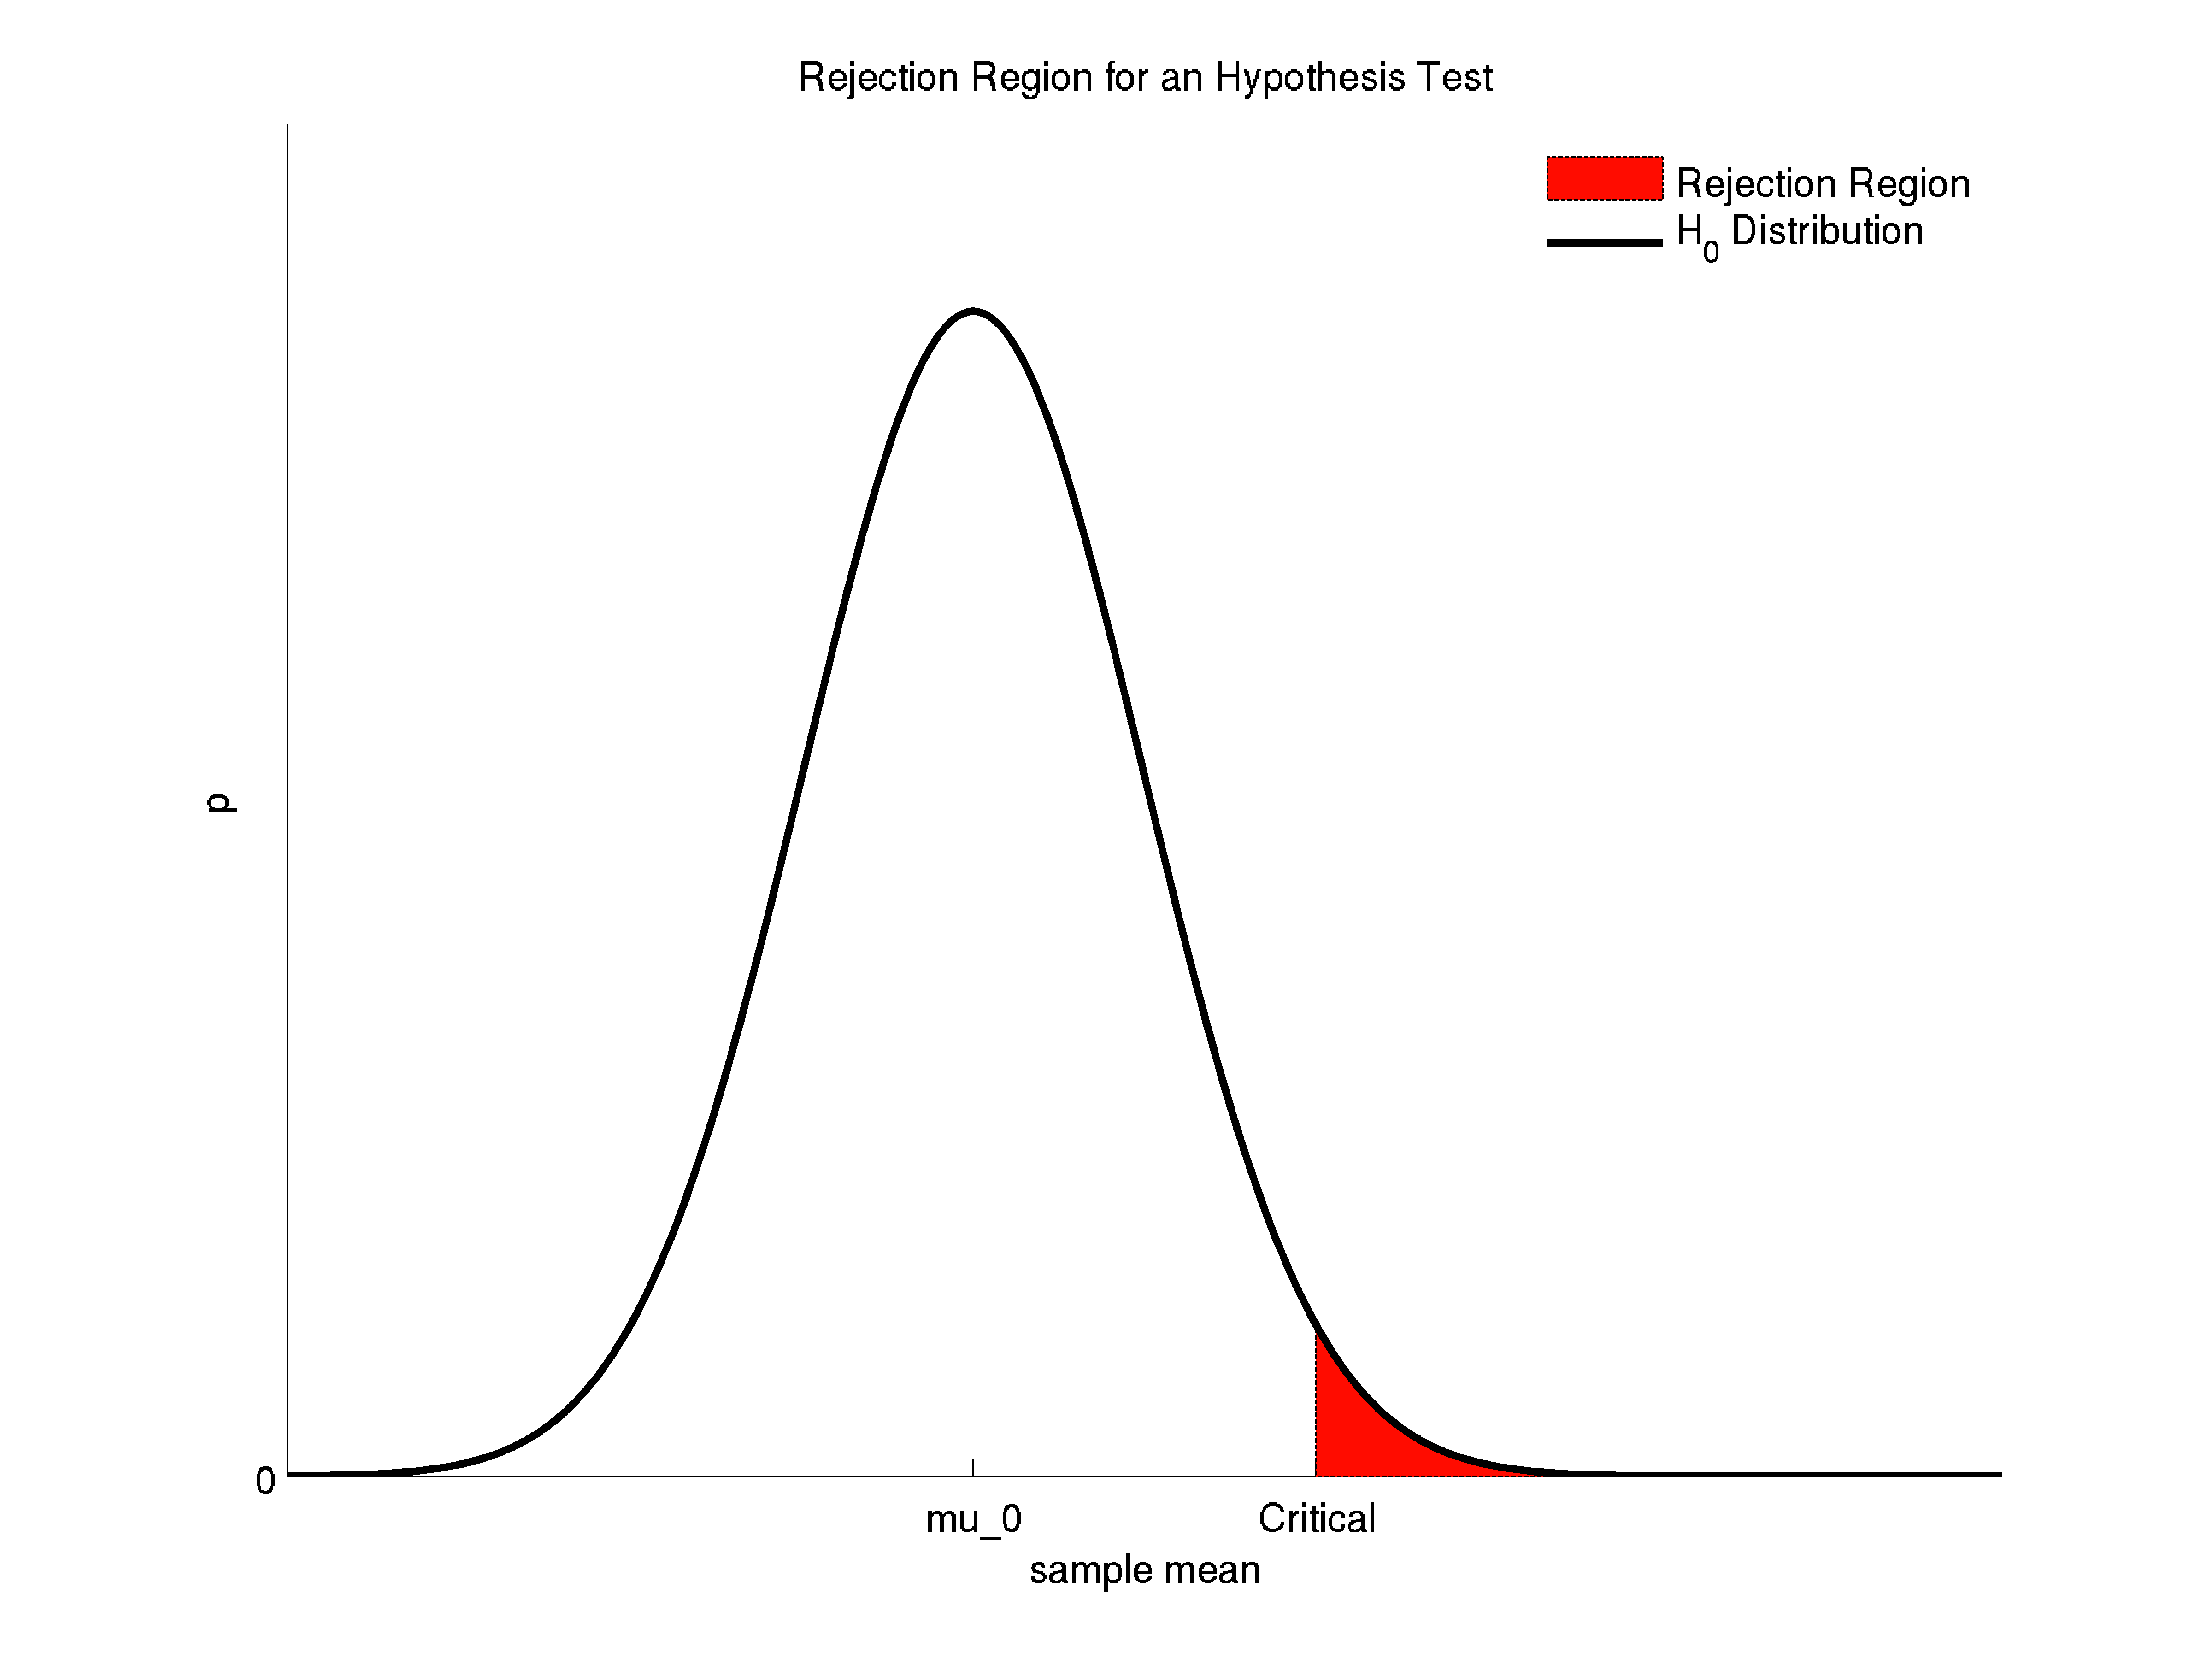
\includegraphics[width=6.0cm]{img/rejectionRegion}}
  }

  \only<2>{
    \centerline{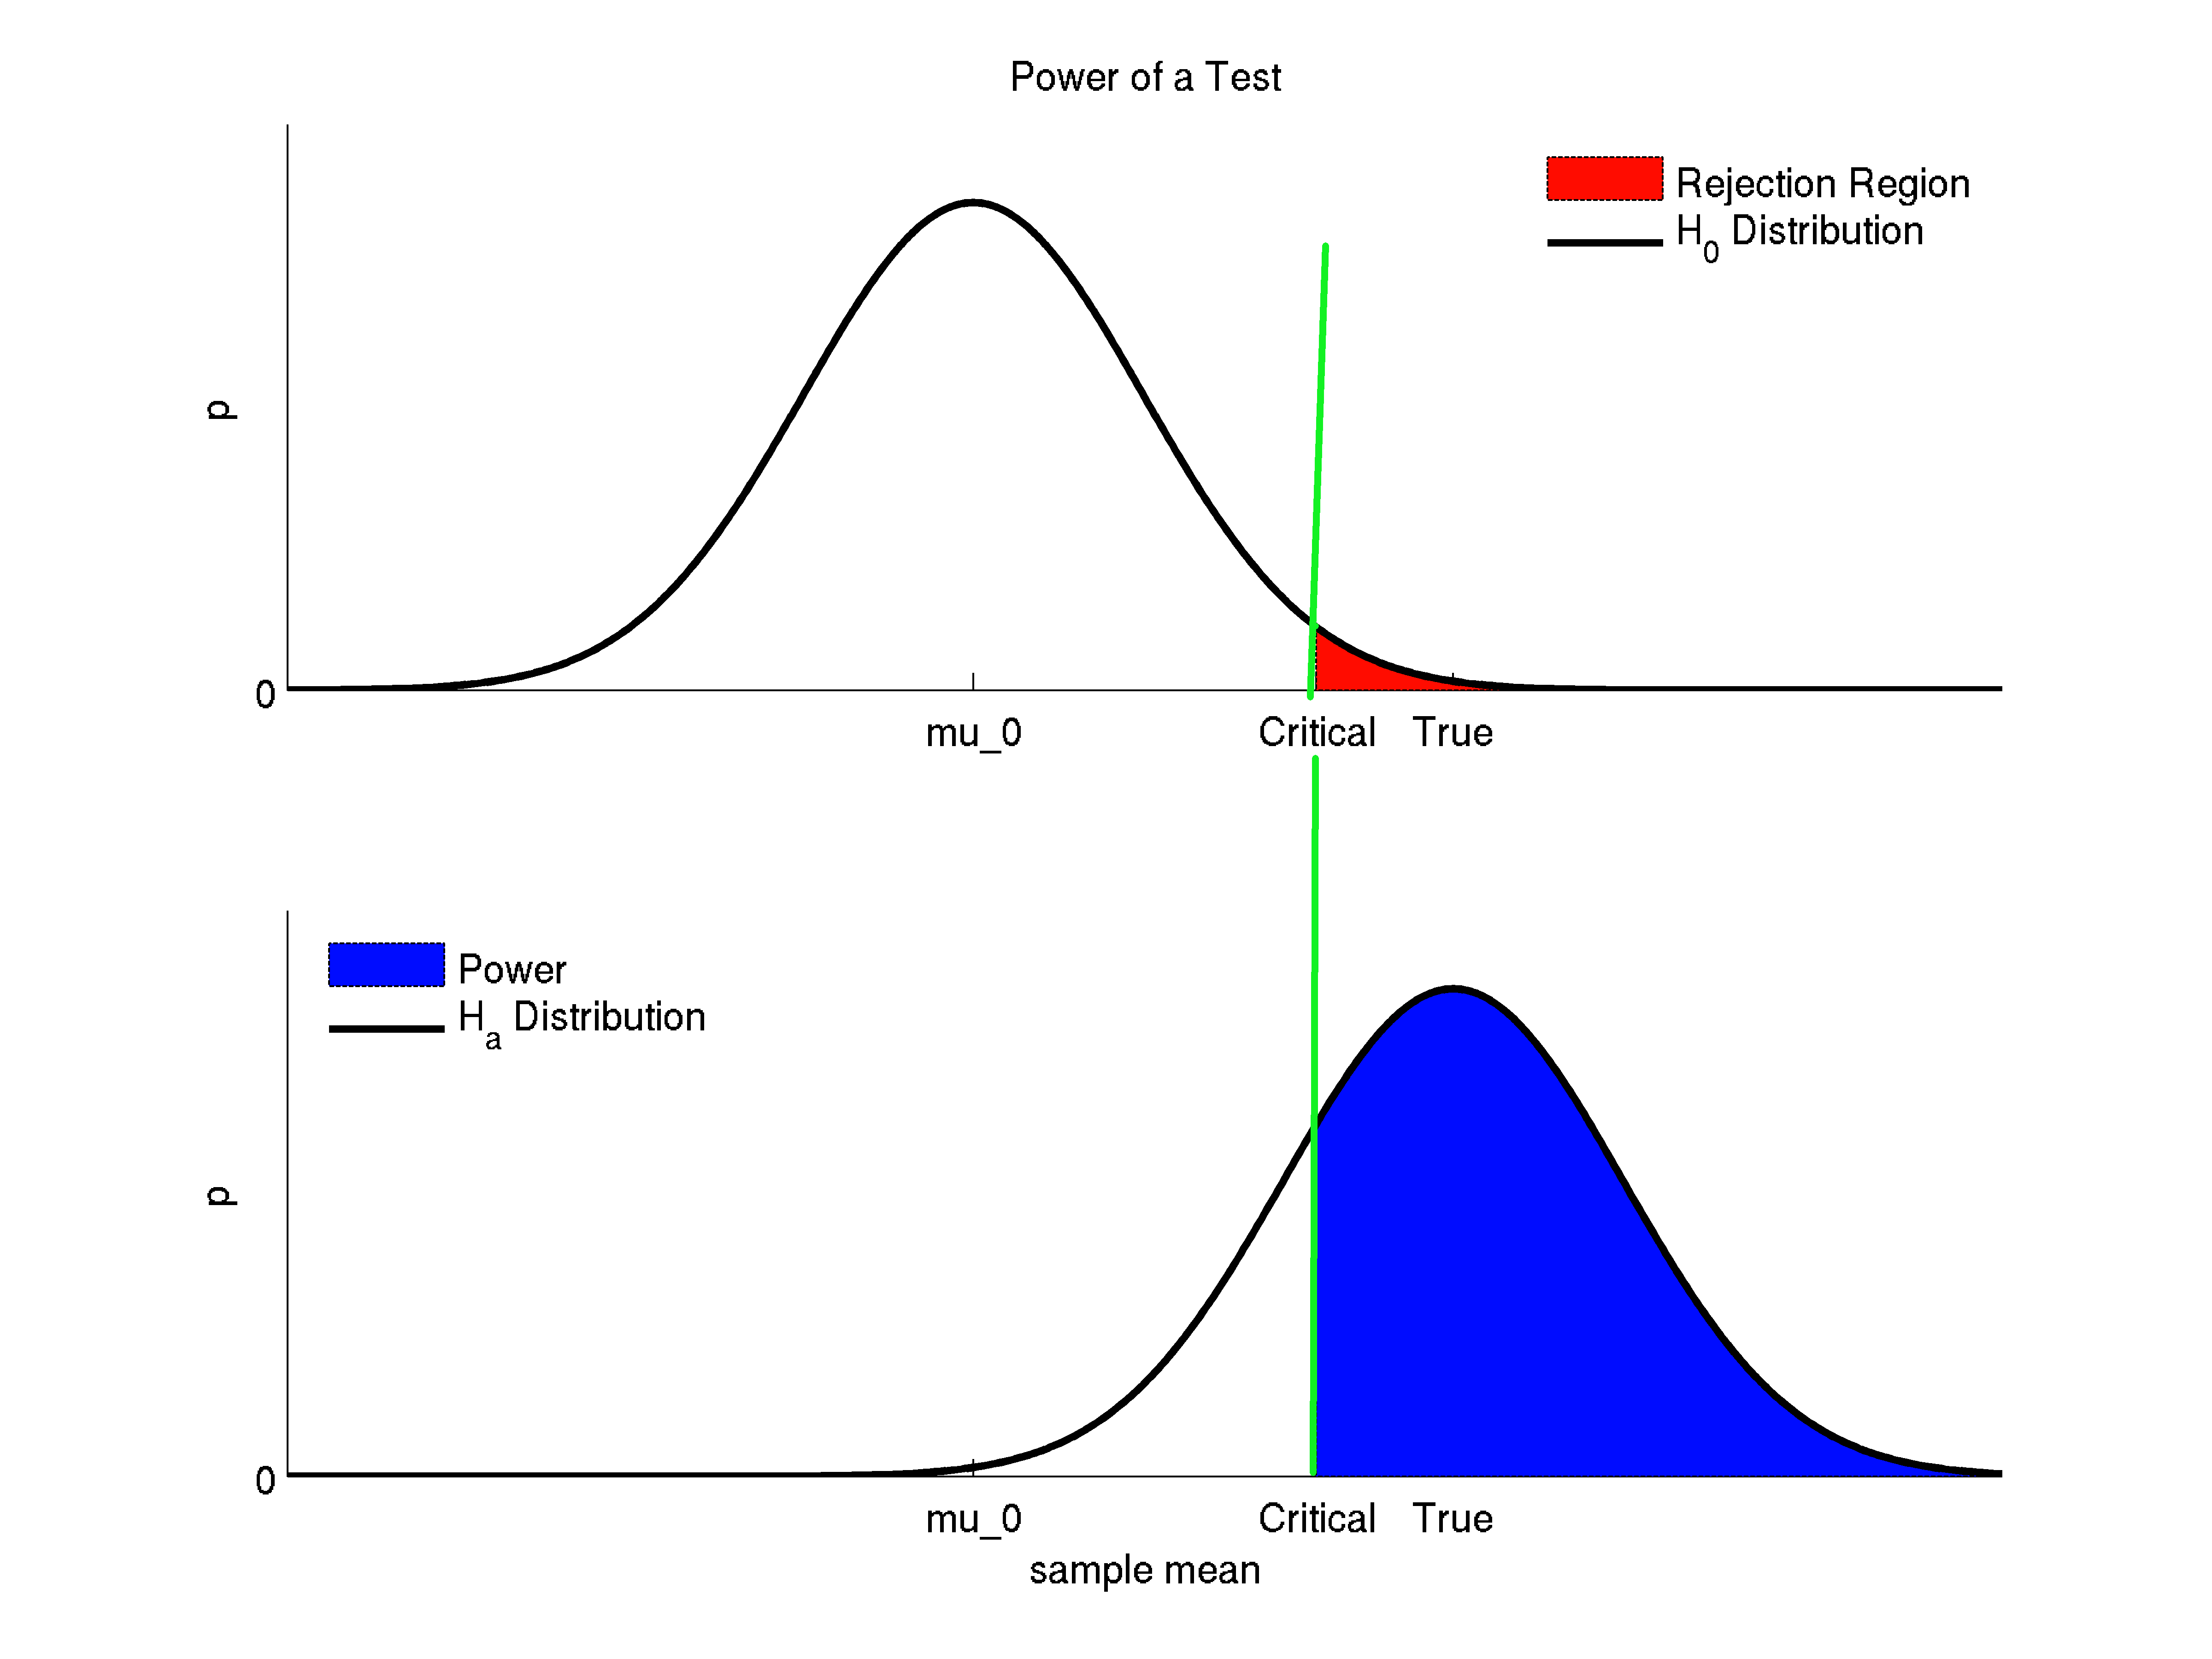
\includegraphics[width=6.0cm]{img/power}}
  }
  
\end{frame}

\begin{frame}{Extra Examples}

  We may or may not cover the following examples in class depending on
  how much time is available.

  \vfill

  You should go over them on your own.

  \vfill
  
\end{frame}

\begin{frame}{Example}

As part of its description of Clarkson, the Princeton Review claims
that the mean height of Clarkson students is 180cm. I think this is
too high and randomly choose a group of students. The following
heights are recorded:

\begin{tabular}{rrrrrrrr}
  148.7 & 181.2 & 168.2 & 173.5 & 169.4 & 170.7 & 163.6 & 173.7 \\
  183.8 & 200.8 & 157.7 & 172.2 & 153.2 & 200.2 & 189.5 & 182.0 \\
  170.7 & 175.3 & 167.2 & 191.4
\end{tabular}

amiright at the 95\% confidence level?

\vfill

\uncover<2->{%

  I cannot reject $H_0$ at the 95\% confidence level assuming a
  $t$-distribution with nineteen degrees of freedom.

  }

\uncover<3->{$p$-value $\approx$ 0.052.}
  
\end{frame}

\begin{frame}{Example}

  I read a brochure about a new area where I will be moving. The
  brochure says that the mean house price is \$285,000. This does not
  seem right, and I choose some houses at random and get the following
  prices:

\begin{tabular}{rrrrrr}
  280000 & 255000 & 307000 & 241000 & 269000 & 265000 \\
  218000 & 198000 & 321000 & 265000 & 239000 & 262000 \\
  301000 & 194000 & 231000 & 337000 & 240000
\end{tabular}

amiright at the 95\% confidence level?

\vfill

\uncover<2->{%

  I can reject $H_0$ at the 95\% confidence level assuming a
  $t$-distribution with sixteen degrees of freedom.

  }

\uncover<3->{$p$-value $\approx$ 0.022.}
  
\end{frame}

\begin{frame}{Example}

  I want to perform the following test:
  \begin{eqnarray*}
    H_0: \mu & = & 800, \\
    H_a: \mu & > & 800, \\
    \alpha & = & 0.05.
  \end{eqnarray*}

  The data yields the following calculations:
  \begin{eqnarray*}
    N & = & 30, \\
    \bar{x} & \approx & 839, \\
    \sigma & = & 118.
  \end{eqnarray*}

  What is the $p$-value, and what is the result?

  \vfill 

  \uncover<2->{%

    The $p$-value is 0.035.

    We can reject $H_0$ at the 5\% significance level assuming a
    normal distribution.

    }
  
\end{frame}


\begin{frame}{Example}

  We will treat a fiber to increase its breaking strength. We expect
  that the standard deviation for the breaking strength of the treated
  fiber will be 8.0N. How many samples will be required to reject the
  null hypothesis if the sample mean is 0.2N greater than the previous
  mean? (Use a 95\% confidence level.)

  \vfill

  \uncover<2->{
    $N=4304$.
  }

  \vfill
  
\end{frame}

\begin{frame}{Example}

  The levels of lead (in PPB) for the water is tested, and the results
  are given below. Determine the 95\% confidence interval.

\begin{tabular}{rrrrrr}
  12.4  & 8.5  & 10.1 & 13.6 & 16.1 & 8.7 \\
  22.4  & 14.6 & 16.4 & 17.9 & 17.2 & 12.4
\end{tabular}


\vfill

\uncover<2->{%

  The 95\% confidence interval is between 11.59 PPB and 16.79 PPB
  assuming a $t$-distribution with eleven degrees of freedom.

}

  
\end{frame}


\begin{frame}{Example}

  The levels of lead (in PPB) for the water is tested, and the results
  are given below. Is the mean level of lead less than 15 PPB? Use a
  confidence interval of 95\%.

\begin{tabular}{rrrrrr}
  12.4  & 8.5  & 10.1 & 13.6 & 16.1 & 8.7 \\
  22.4  & 14.6 & 16.4 & 17.9 & 17.2 & 12.4
\end{tabular}


\vfill

\uncover<2->{%

  The null hypothesis cannot be rejected at the 95\% confidence level
  assuming a $t$ distribution with eleven degrees of freedom.

}

\uncover<3->{%

  The $p$-value is approximately 0.25.

}

  
\end{frame}



% LocalWords:  Clarkson pausesection hideallsubsections hideothersubsections
% LocalWords:  sectionstyle
